\section{Obstacle Avoidance}

\subsection*{(c)}
At SCP iteration \(i\), the cost is already convex, so only the dynamics and
obstacle constraints are replaced by affine approximations. The convex
subproblem is
\[
\begin{aligned}
\min_{s_{\cdot|t},u_{\cdot|t}}\quad
& (s_{N|t}-s_{\rm goal})^TP(s_{N|t}-s_{\rm goal})
+ \sum_{k=0}^{N-1}
\left[
(s_{k|t}-s_{\rm goal})^TQ(s_{k|t}-s_{\rm goal})
+ u_{k|t}^TRu_{k|t}
\right] \\
\text{s.t.}\quad
& s_{0|t}=s(t) \\
& s_{k+1|t}
= A_{f,k|t}^{(i)}s_{k|t}
+ B_{f,k|t}^{(i)}u_{k|t}
+ c_{f,k|t}^{(i)},
\quad k=0,\ldots,N-1 \\
& A_{d,k|t}^{(i)}s_{k|t}
+ c_{d,k|t}^{(i)} \succeq 0,
\quad k=0,\ldots,N
\end{aligned}
\]
where
\[
\begin{aligned}
A_{f,k|t}^{(i)}
&=
\left.\frac{\partial f}{\partial s}\right|_
{(s_{k|t}^{(i)},u_{k|t}^{(i)})} \\
B_{f,k|t}^{(i)}
&=
\left.\frac{\partial f}{\partial u}\right|_
{(s_{k|t}^{(i)},u_{k|t}^{(i)})} \\
c_{f,k|t}^{(i)}
&=
f(s_{k|t}^{(i)},u_{k|t}^{(i)})
- A_{f,k|t}^{(i)}s_{k|t}^{(i)}
- B_{f,k|t}^{(i)}u_{k|t}^{(i)} \\
A_{d,k|t}^{(i)}
&=
\left.\frac{\partial d}{\partial s}\right|_{s_{k|t}^{(i)}} \\
c_{d,k|t}^{(i)}
&=
d(s_{k|t}^{(i)})
- A_{d,k|t}^{(i)}s_{k|t}^{(i)}
\end{aligned}
\]


\subsection*{(d)}
Each signed distance \(d_j(s)\) is convex, so its first-order Taylor approximation is a global lower bound:

% \[
% d_j(s) \ge d_j(\bar s)
% + \nabla d_j(\bar s)^T(s-\bar s)
% \]
% The affine approximation can be written as
% \[
% A_{d,j}^{(i)}s+c_{d,j}^{(i)}
% =
% d_j(\bar s)
% + \nabla d_j(\bar s)^T(s-\bar s)
% \]
% Therefore, if the SCP constraint enforces
% \[
% A_{d,j}^{(i)}s+c_{d,j}^{(i)} \ge 0
% \]
% then
% \[
% d_j(s) \ge A_{d,j}^{(i)}s+c_{d,j}^{(i)} \ge 0
% \]
% So satisfying the affine constraint is conservative, but it guarantees the
% true obstacle constraint.


\subsection*{(g)}

\[
\begin{array}{c|c|c|c}
N & N_{\mathrm{SCP}} & \text{total time (s)} & \text{total control cost}\\
\hline
5 & 5 & 20.30 & 6.93\\
2 & 5 & 18.80 & 11.18\\
5 & 2 & 11.81 & 4.43\\
15 & 2 & 14.49 & 4.50
\end{array}
\]

\begin{figure}[H]
    \centering
    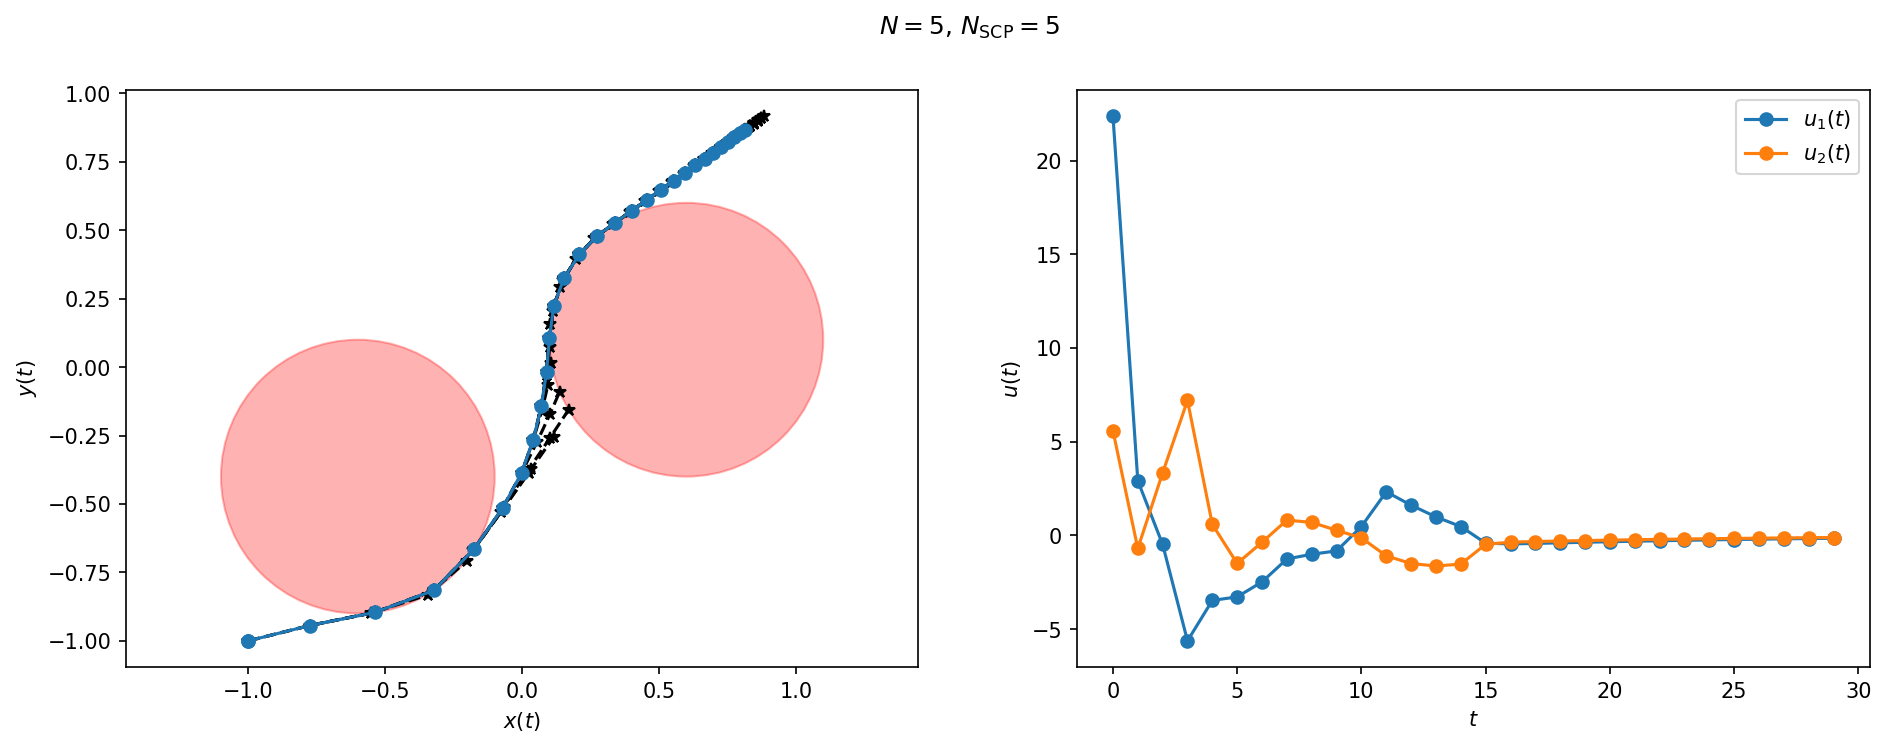
\includegraphics[width=\textwidth]{figures/soln_obstacle_avoidance_N=5_Nscp=5.png}
\caption{\(N=5,\ N_{\mathrm{SCP}}=5\)}
\end{figure}

With \(N=5\) and \(N_{\mathrm{SCP}}=5\), the trajectory avoids both obstacles and
is reasonably smooth. This case takes the most time because each MPC solve uses
more SCP iterations.

\begin{figure}[H]
    \centering
    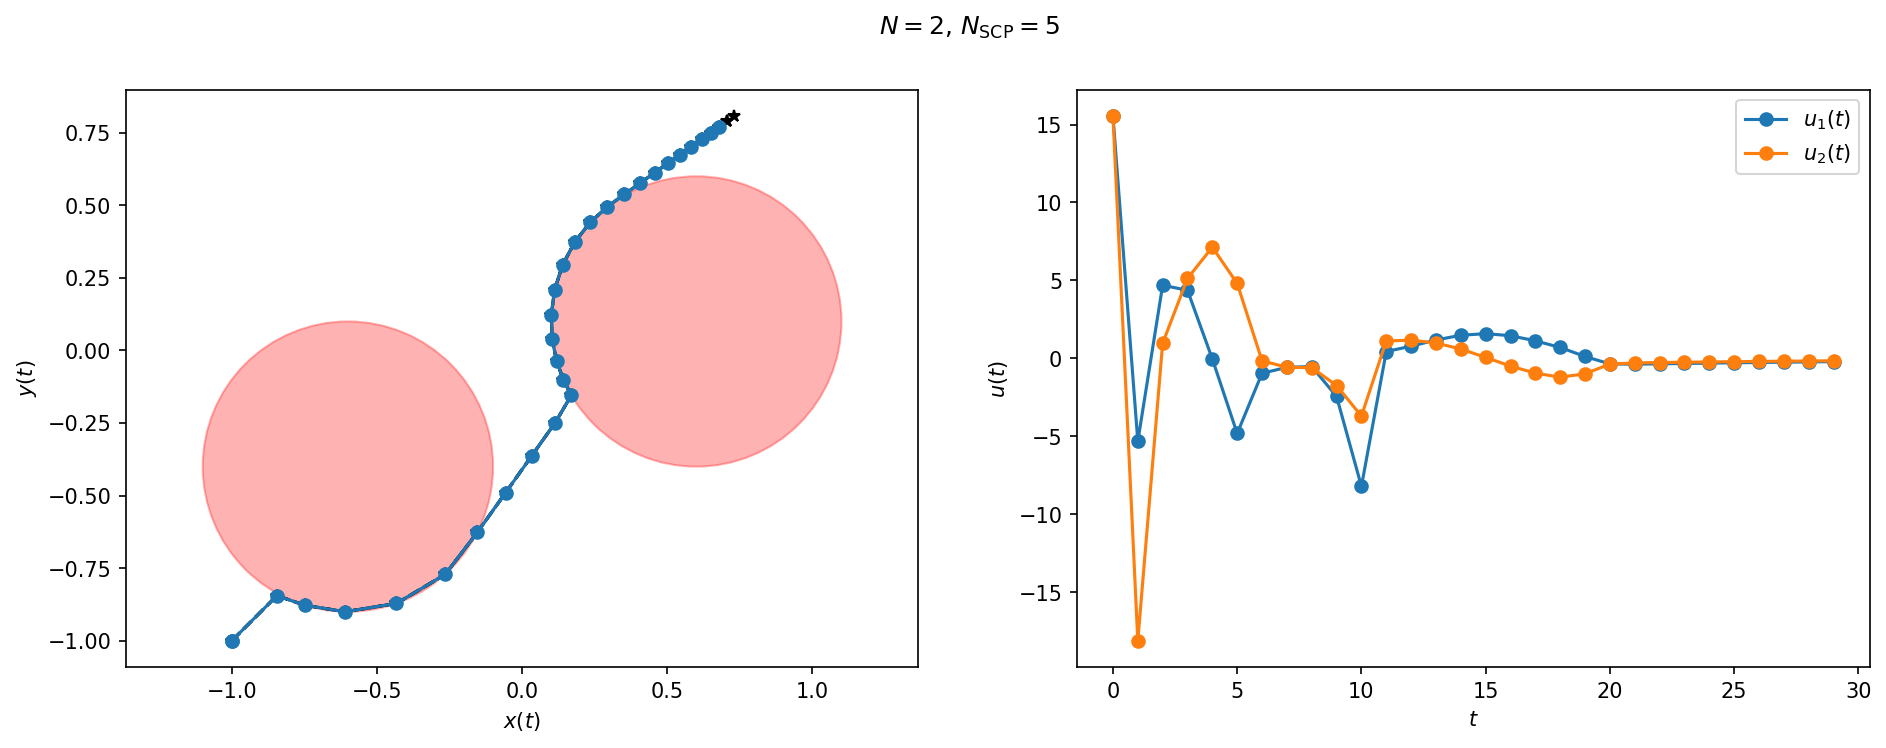
\includegraphics[width=\textwidth]{figures/soln_obstacle_avoidance_N=2_Nscp=5.png}
\caption{\(N=2,\ N_{\mathrm{SCP}}=5\)}
\end{figure}

With \(N=2\), the controller is much more short-sighted. It still avoids the
obstacles, but the path and controls are less smooth, and the total control cost
is the largest.

\begin{figure}[H]
    \centering
    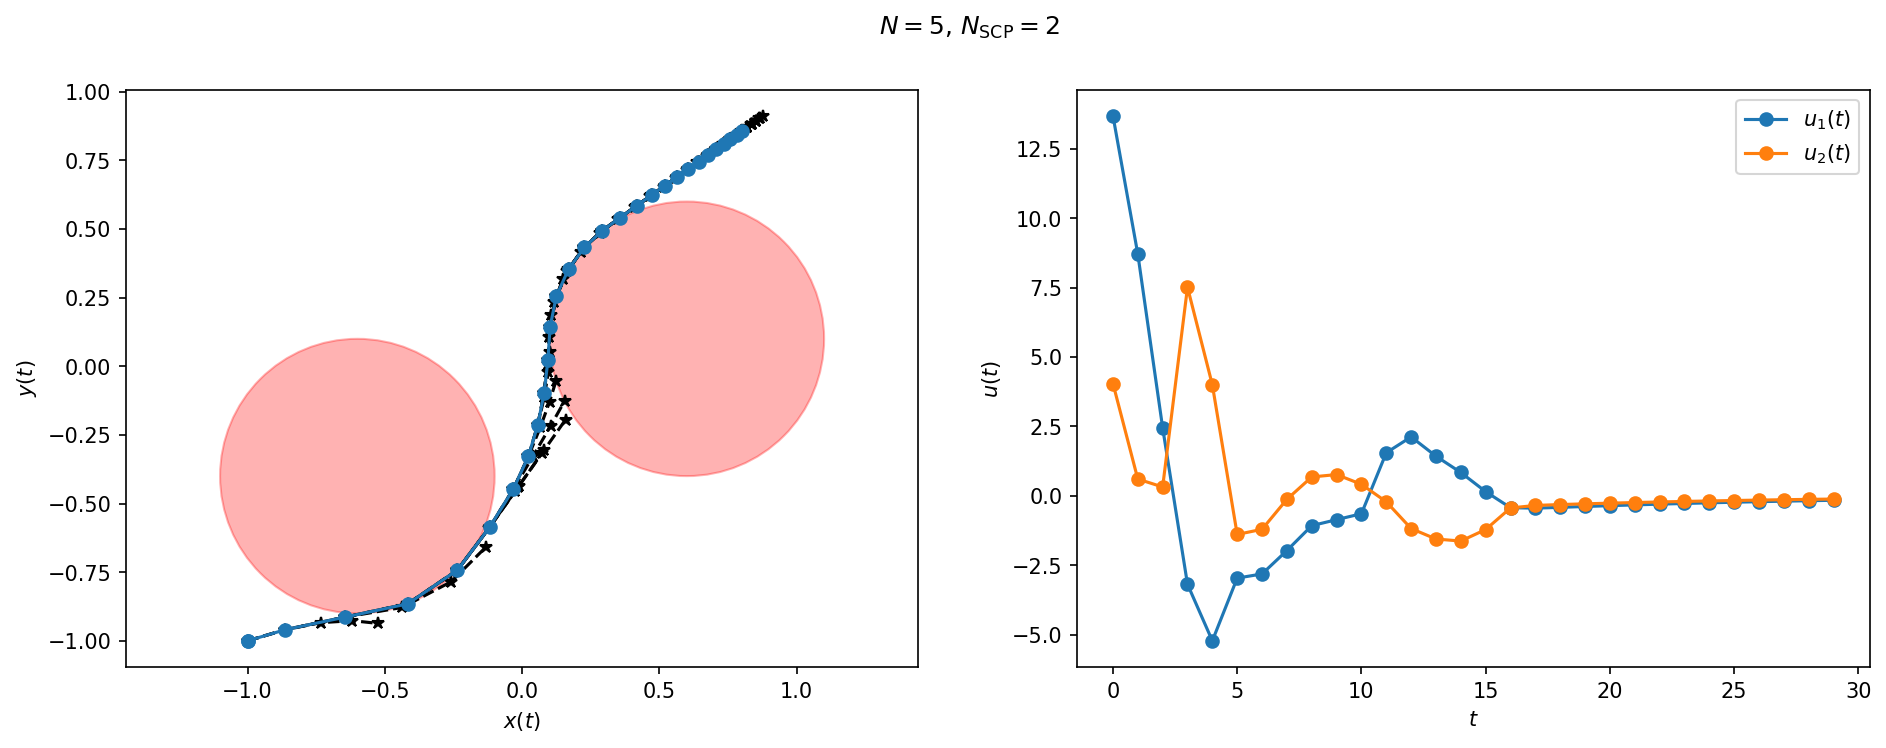
\includegraphics[width=\textwidth]{figures/soln_obstacle_avoidance_N=5_Nscp=2.png}
\caption{\(N=5,\ N_{\mathrm{SCP}}=2\)}
\end{figure}

With \(N=5\) and only two SCP iterations, the computation time drops a lot while
still giving a good trajectory. In this run it also gives the lowest control
cost.

\begin{figure}[H]
    \centering
    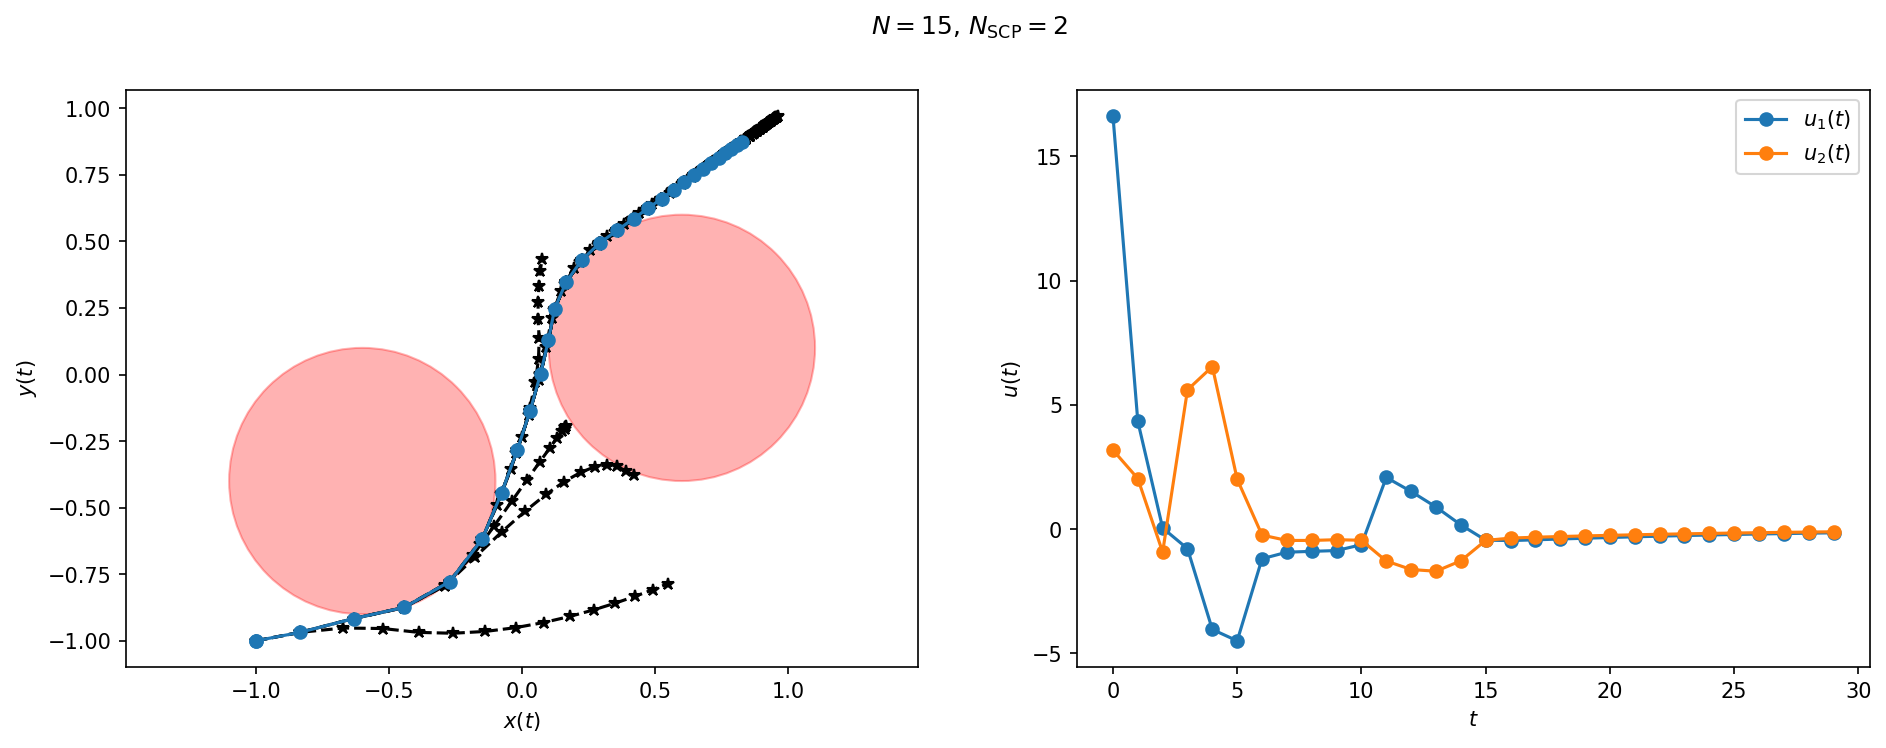
\includegraphics[width=\textwidth]{figures/soln_obstacle_avoidance_N=15_Nscp=2.png}
\caption{\(N=15,\ N_{\mathrm{SCP}}=2\)}
\end{figure}

With \(N=15\), the planned trajectories are smoother because the controller can
see farther ahead. The solve time is higher than \(N=5,\ N_{\mathrm{SCP}}=2\),
but the control cost is still low.
